%%% PGCONF.EU 2012, Prague
%%%
%%% Lightning Talk: PGQ Cooperative Consumers

\documentclass{beamer}

\usepackage{beamerthemesplit}
%% \usetheme{Warsaw}
\usetheme{Frankfurt}
\beamertemplatetransparentcovered

\title{PGQ Cooperative Consumers}
\author{Dimitri Fontaine \newline\tiny{\texttt{dimitri@2ndQuadrant.fr}}}
\date{25 Oct. 2012}
\logo{
\includegraphics[height=0.4cm]{2ndQuadrant-cross.png}}

\begin{document}

\frame{\titlepage}

\section{Batches needs}

\begin{frame}[fragile]
  \frametitle{Database processing oriented batches}

\begin{columns}[c]

\column{.5\textwidth}

If you're managing an \textit{OLTP} system, you probably have out of line
processing to get done, and probably are using cron batches and home made
\textit{daemons}.

\pause
\begin{example}
\begin{verbatim}
  while True: 
    // what a nice daemon!
\end{verbatim}
\end{example}

\pause
\column{.5\textwidth} 
  Of course you want them 
  \begin{itemize}
   \item<3-> reliable, easy to monitor and control (logs)
   \item<4-> out of a developer \texttt{screen} session
   \item<5-> easy to stop \& restart
   \item<6-> to reuse existing models
  \end{itemize}

\end{columns}
\end{frame}

\section{PGQ features}

\begin{frame}[fragile]
  \frametitle{Queueing with \textit{PGQ}}

  \center{\textit{Off-line} processing is better done with \texttt{PGQ}}
  \linebreak

\begin{columns}[c]
\column{.6\textwidth} 

  \begin{itemize}
   \item Mainly written in \texttt{PLpgSQL} (and \texttt{C})
   \item Client \textit{API} for \texttt{python}
   \item and \texttt{PHP}
   \item some work is happening for \texttt{Java}
   \item \textbf{Cooperative Worker} (Skytools 3)
  \end{itemize}  

  \onslide<2->{\center{\texttt{PGQ}: Stable, Reliable, Easy to monitor}}

\column{.4\textwidth}

\includegraphics[height=9em]{drop-queue.png}
\end{columns}
\end{frame}

\section{Mix and Match}

\frame{
  \frametitle{Implementing a daemon atop PGQ}

  Skytools comes with two \textit{middleware} for you to abuse to make
  daemons with, the \texttt{python} \textit{DBScript} facility and the
  \texttt{PHP} \textit{libphp-pgq} one.

\begin{columns}[c]
\column{.6\textwidth} 

  \begin{itemize}
    \item \texttt{skytools3}
    \item \texttt{python-pgq3}
    \item \texttt{python-skytools3}
    \item \texttt{skytools-ticker3}
    \item \texttt{skytools-walmgr3}
    \item \texttt{postgresql-8.4-pgq3}
    \item \texttt{postgresql-9.0-pgq3}
  \end{itemize}

\column{.4\textwidth}

\includegraphics[height=9em]{pydebian.png}
\end{columns}
}

\begin{frame}[fragile]
  \frametitle{Several Kinds of Consumers}

  Some consumers will only offload local processing, some are maintaining
  \textit{remote} data when processing events from the local queue.

  \begin{itemize}
   \item PGQ Consumer, single connection
   \item PGQ Remote Consumer, two connections
   \item PGQ Cooperative Consumer, one connection
  \end{itemize}
\end{frame}

\section{Going Live!}

\begin{frame}[fragile]
  \frametitle{Monitoring Cooperative Consumers}

\begin{center} 
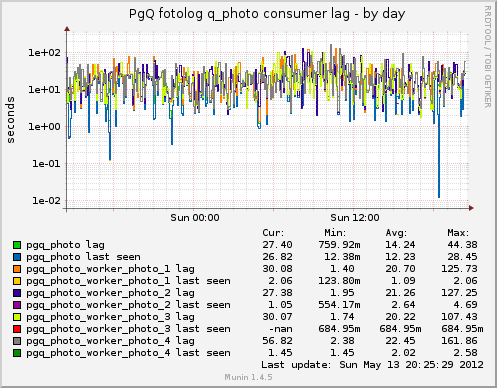
\includegraphics[height=2.1in]{pg_queue_fotolog_q_photo-day.png}
\end{center} 
\end{frame}

\begin{frame}[fragile]
  \frametitle{Managing production daemons}

  We have several \texttt{PGQ} daemons in our live environments, monitored
  with \texttt{nagios} and \texttt{munin}, and we're able to easily control
  them. It's much better than previously.

\begin{columns}[c]
\column{.5\textwidth}
  \begin{example}[PHP daemon management example]
  \begin{verbatim}
    # mydaemon.php start
    # mydaemon.php status
    # mydaemon.php logmore

    # mydaemon.php kill
  \end{verbatim}
  \end{example}
\column{.5\textwidth} 
\begin{center} 
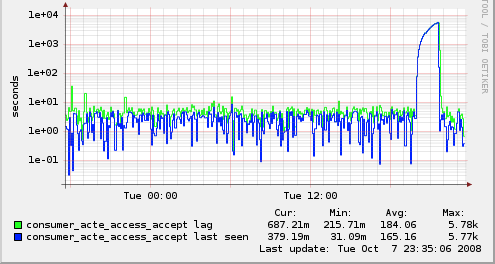
\includegraphics[height=1.3in]{pgq.png}
\end{center} 
\end{columns}
\end{frame}

\end{document}
